\documentclass[aps,prl,twocolumn,superscriptaddress]{revtex4-1}

% the percent sign gives comments in Latex
% top line indicates this is for Physical Review, standard journal format,
% suitable for electronic submission of articles
%
% the line above is necessary to start any latex document.
% this is one variation that should work for most things.
% if you want double spaceing, use the following:
%
%\documentclass[prd,preprint,letterpaper]{revtex4}
%
% the "preprint" designation will make a wider line
% spacing, good for markup.
\usepackage{graphicx}  % this is the up-to-date package for all figures
\usepackage{amssymb}   % for math
\usepackage{verbatim}  % for the comment environment
\usepackage{color}
\usepackage{float}	% allows use of 'H' command
%\usepackage{hyperref}	% needed to add hyperlinks
%\hypersetup{
%  colorlinks=true,
%  linkcolor=blue,
%  filecolor=magenta,
%  urlcolor=cyan,
%}
\bibliographystyle{apsrev}


% these are some custom control of the page size and margins
% \topmargin= 0.2in  % these 1st two may be needed for some computers
% \textheight=8.75in
\textwidth=6.5in
%\oddsidemargin=0cm
%\evensidemargin=0cm

% this is where the actual document itself (rather than control statements) begins:

\begin{document}



\title{Modeling Schr\"{o}dinger's Equation: \\
Numerical Solutions}


\author{Steve Covin}
\author{Corey Mutnik}
\email{spicer2@hawaii.edu}
\email{cmutnik@hawaii.edu}
\affiliation{Department of Physics \& Astronomy, \\
University of Hawaii at Manoa,\\
2505 Correa Rd, Honolulu, HI, 96822, USA}
\altaffiliation{Computational Physics 305}



	      % \section is used to start a new one with a heading
\begin{abstract}
This study produces numerical solutions to the Shr\"{o}dinger equation. The allowed energy states of particles and the corresponding wavefunctions was simulated for the case of a quantum harmonic oscillator, as well as an approximation of a hydrogen atom modeling electrons bound to a nearby proton. The Numerov algorithm we used was validated by comparing the results of these simulations to their analytical solutions, and extrapolated to generate information about an electron near a diatomic hydrogen molecule. 

\end{abstract}

\maketitle    


\section{Introduction and Overview}

In introductory quantum mechanics classes students are 
exposed to the particle in a box thought experiment, in which  
one imagines square potential well of finite length.  Within the bounds of 
this well the potential is zero, any particle is classically allowed to be in this region.  For any distance beyond the 
length of the well, on either side, the potential infinitely high, thus no particle can have enough energy to move into this region.  These regions are refered to as the classically "forbidden regions".
Such forbidden regions are not restricted to square wells.  Any position where the potential energy function in that region is higher than the kinetic energy of the particle is classically forbidden. However quantum mechanics tells us that a particle can 
exist where it classically should not be able to.  This is indicated by it's probability 
density being nonzero in these regions.


The probability density to find a particle in a given region is described by the wavefunction associated with it's energy level. In order to determine it's wavefunction, we must use the Schr\"{o}dinger 
equation.  The aim of this project %paper??????????experiment????
is to simulate quantum wavefunctions and probability densities using 
numerical/computational methods.  By doing this we were able to show the likelihood 
that a particle would exist outside the potential well encasing it.


Initially we aimed to simulate analytically solvable potentials.  The first situation we 
modeled was that of a one-dimensional, time-independent, quantum harmonic oscillator.  Once the accuracy of our program was verified, we extended it to simulate the case of a two-dimensional oscillator.  Using 
the same methodology a program modeling coulombic potentials was written.  Finally, a program 
that simulates the potential well of diatomic hydrogen was generated.  In order to do this we 
implemented Numerov's algorithm, an advanced numerical technique.  

\section{Description of Computational Problem}

In this study we numerically integrate the time independent Shr\"{o}dinger equation, a partial differential equation that 
describes the quantum state of a physical system. The solution depends on the total energy of the system; specifically the 
kinetic energy of the particle whose wavefunction we wish to determine, as well as the potential energy function in the 
vicinity of the particle. Although analytical solutions do exist for many systems, more complicated interactions between the 
particle and its surroundings often require numerical solutions. 

The computational approach to this problem is to discretize Shr\"{o}dinger's equation onto a grid of finite resolution and 
evaluate the solution based on a series of educated guesses. For this we used Numerov's method, named for Russian astronomer 
Boris Numerov~\cite{comparison}. This method is optimized to integrate second-order differential equations of the form:
 $$\frac{d^2y(x)}{dx^2}+a(x)y(x) = 0$$
 for some known function $a(x)$. We can write Shr\"{o}dinger's equation in this form as shown in Eq.~(\ref{psiF}).

\subsection{Contributing factors.}

The quantization of energy levels in bound states is a requirement for a physically significant solution, which arise from the 
boundary conditions of the system. Numerov's algorithm can produce a waveform for any energy, but it may not describe a 
physically real system. If the energy level used to evaluate $\psi$ does not correspond to the correct energy level, $\psi$ will 
diverge. However, $\psi$ and the corresponding energy level are both unknown in this problem. In linear algebra terms, they 
describe an eigenfunction and corresponding eigenvalue.

\subsubsection{The Shooting Method.}

Some amount of guessing is required to arrive at the solution to this problem. For a bound state the energy level must be within 
the potential well, so we can begin searching in the middle of the upper and lower limits of the potential energy 
levels; $E = (E_{max}-E_{min})/2$. If the waveform drawn by Numerov's algorithm using this energy level diverges to 
some $E>0$, or if it has more nodes than the quantum state we wish to describe, then we know the eigenvalue must be in the 
lower interval. Conversely, we can also determine if the eigenvalue is in the upper interval. We continue ``shooting" waveforms 
until we either have a converging solution with the correct number of nodes, the gap between $E_{max}$ and $E_{min}$ reaches a 
pre-determined minimum threshold, or any of several possible failure states occur. 

\subsubsection{The Bisectional Approach.}

One such failure state can be avoided with some careful design. The Shr\"{o}dinger equation is sensitive to small variations 
in $E$, and small perturbations can cause $\psi$ to diverge. As a result, when integrating outward at large distances from the 
origin, the accumulated errors from the Numerov approximation can cause $\psi$ to diverge even for the correct eigenvalue. To 
account for this, we use the knowledge that no nodes can occur in the classically forbidden region, which only decays 
exponentially. Using the shooting method, we integrate $\psi_L$ outwards in the allowed region only, adjusting $E$ until the 
correct number of nodes is achieved. Then $\psi_R$ is integrated backwards in the forbidden region, and rescaled to match the 
value of $\psi_L$ at the classical limit. The smoothness of the function at this junction can also help converge on the 
eigenvalue; if $\psi'_R-\psi'_L>0$ the energy is too high, and we can choose choose the upper or lower energy interval accordingly. 

\subsection{Numerov Algorithm.}

The Numerov algorithm is specifically tailored for solving the Schr\"{o}dinger 
equation.  For this reason it is exceptionally more accurate and efficient 
than any other numerical method.  For this reason, our programs implement 
the Numerov algorithm.  Its derivation is shown below.



In order to obtain the desired recursion we must first manipulate the Schr\"{o}dinger 
equation, Eq.~\ref{SWE}, so it takes the form:
\begin{equation}
 \psi^{(2)}(x) + F(x) \psi(x) = 0	\label{psiF}
\end{equation}
In this context an exponent enclosed in parentheses denotes a spatial derivative with respect to x, $\psi(x)$ is 
the one-dimensional wave function and
%\begin{center}
$$F(x) = \frac{2m}{\hbar^2}(E-V(x)).$$
%\end{center}
Where m is the mass of the particle, $\hbar$ is the reduced Plancks's constant, E is 
the total energy, and V(x) is the potential energy.\\
The next step is to approximate $\psi (x \pm h)$ using a Taylor series expansion~\cite{Javapsi}:

 
\begin{center}

$\psi(x+h)=\psi(x) + h \psi^{(1)}(x) + \frac{h^2}{2} \psi^{(2)}(x) + \frac{h^3}{6} \psi^{(3)}(x)+\frac{h^4}{24}\psi^{(4)}(x)+...$
\end{center}
%\\
\begin{center}
$\psi(x-h)=\psi(x)-h\psi^{(1)}(x)+\frac{h^2}{2}\psi^{(2)}(x)-\frac{h^3}{6}\psi^{(3)}(x)+\frac{h^4}{24}\psi^{(4)}(x)-...$
\end{center}
where h is an incremental change, not Planck's constant.\\
Next we take the sum of these two terms:
\begin{center}
$\psi(x+h)+\psi(x-h) = 2\psi(x) + h^2\psi^{(2)}(x) + \frac{h^4}{12}\psi^{(4)}(x)+O(h^6)$	\label{3.3}
\end{center}

By rearraging terms in the previous equation we arrive at:
\begin{center}
$\psi(x+h) = -\psi(x-h)+2\psi(x)+h^2\psi^{(2)}(x) + \frac{h^4}{12}\psi^{(4)}(x) + O(h^6)$
\end{center}
Eq.~\ref{psiF} gives us $\psi^{(2)}(x)$ and allows us to solve for $\psi^{(4)}(x)$:
%\begin{center}
$$\psi^{(4)}(x) = \frac{d^2}{dx^2}(-F(x)\psi(x))$$
%\end{center}
%\\
%Finally we insert the obtained values into Eq.~\ref{3.3} and arrive the desired iteration,
Finally we arrive at the desired iteration,
\\
\begin{center}
$\psi(x+h) = \frac{\psi (x) [2-\frac{5h^2}{6} F(x)] - \psi (x-h)[1+\frac{h^2}{12}F(x-h)]}{1+\frac{h^2}{12}F(x+h)}$
\end{center}

allowing the algorithm to make the necessary calculations.

\subsubsection{Numerov Applied to Higher Dimensions.}

In order to use numerov in calculating the value of $\psi$ in more than one dimension, iterations in each direction must 
be accounted for. For the two-dimensional, time-independent case:
\\
\begin{center}
$\psi(x,y) = \frac{\psi(x+h,y) + \psi(x-h,y) + \psi(x,y+h) + \psi(x,y-h)}{4-h^2F(x,y)}$
\end{center}

\section{Schr\"{o}dinger's Equation}

For any quantum mechanical system the wave function, $\psi$, must be solved for, before one is able to 
calculate the position probability density of a corresponding particle~\cite{Javapsi}.  In order to do this one must solve 
the Schr\"{o}dinger equation, devised by Erwin Schr\"{o}dinger in 1926~\cite{Schrodinger_wave}.
\begin{equation}
 E\Psi(\vec r) = [\frac{\hbar^2}{2\mu}\vec\nabla^2 + V(\vec r)]\Psi(\vec r)	\label{SWE}
\end{equation}
where $V$ is the potential energy function, $\nabla$ is the gradient operator, and $\mu$ is the reduced mass of the system:
$$\frac{m_1m_2}{m_1+m_2}$$
This equation models the wave function of a particle in three spatial dimensions~\cite{Sch_eq}.

\section{Quantum Harmonic Oscillator}

      \subsection{One-dimensional, time-independent case.}

The Schr\"{o}dinger equation for a one-dimensional harmonic oscillator is:
\begin{equation}
\frac{d^2\psi(x)}{dx^2} = -\frac{2m}{\hbar}[E-V(x)]\psi(x) \label{harmSh}
\end{equation}
where 
$$V(x) = \frac{1}{2}Kx^2.$$
This approach models the particle as a mass on a spring, which experiences a restoring force $F = -Kx$ from a central 
equilibrium point. Classically, the particle has angular frequency:
\begin{equation}
\omega = \sqrt{\frac{K}{m}}. \label{freq}
\end{equation}
In order to simplify the problem, we introduce adimensional variables $\xi$, $x$ and $\epsilon$:
$$\xi \equiv (\frac{mK}{\hbar^2})^{1/4}$$
$$x \equiv (\frac{m\omega}{\hbar})^{1/2}x$$
$$\epsilon \equiv \frac{E}{\hbar\omega}$$
Then Eq.~(\ref{harmSh}) becomes a function of $\xi$:
\begin{equation}
\frac{d^2\psi(\xi)}{d\xi^2} = -2(\epsilon-\frac{\xi^2}{2})\psi(\xi) \label{shroxi}
\end{equation}
For large $\xi$, the squared term dominates and the equation above becomes asymptotic:
\begin{equation}
\psi(\xi) \rightarrow \xi^ne^{-\xi^2/2} \label{largexi}
\end{equation}
Eq.~(\ref{largexi}) produces nondiverging solutions when
\begin{equation}
\epsilon = n+\frac{1}{2},~n=0,1,2,...
\end{equation}
Then the nth bound state in the quantum harmonic oscillator has quantized energy levels~\cite{code}:
\begin{equation}
E_n = \hbar \omega (n+\frac{1}{2}),~n=0,1,2,... \label{harmE}
\end{equation}
and the complete wavefunction associated with energy $E_n$ is~\cite{Schrodinger_wave}:
\begin{equation}
 \psi_{n}(\xi) = H_{n}(\xi) e^{-\xi^2/2}
\end{equation}
where $H_n$ are Hermite polynomials of order $n$:
$$H_{n}(x) = (-1)^n e^{x^2} \frac{d^n}{dx^n}(e^{-x^2})$$

We use the analytic solutions for $E_n$ and the corresponding $\psi_n$ to compare with predictions made by Numerov's 
method, in order to determine the accuracy of the algorithm. 

\begin{figure}[h!]
 \centering
 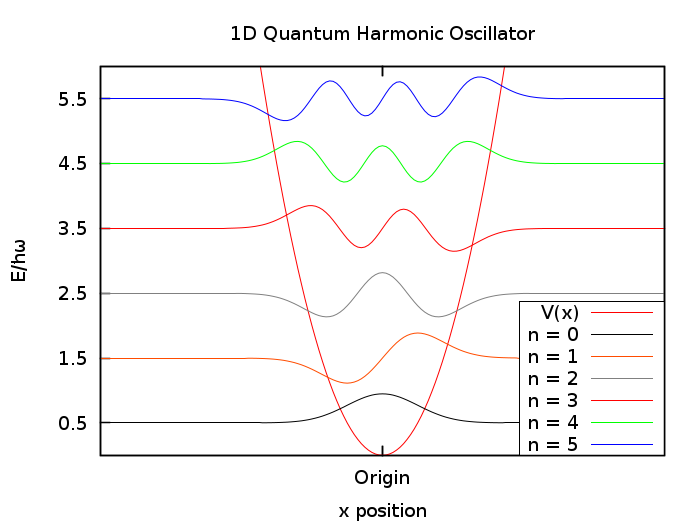
\includegraphics[width=3.35in]{harmOsc.png}
 % harmOsc.png: 0x0 pixel, 300dpi, 0.00x0.00 cm, bb=
 \caption{\it \small{The wavefunctions associated with the first six bound eigenstates, $n$=0 to 5, as generated by Numerov's algorithm.}}
 \label{fig:harmOsc}
\end{figure}

\begin{table}[h!]
\label{data}
\begin{center}
\begin{tabular}{|c|c|c|c|} 
\hline
n  & Predicted $E_n$  & Simulated $E_n$    & Fractional Error \\
\hline\hline
0  & $\frac{1}{2}\hbar\omega$ & $0.500000035\hbar\omega$ & $7.0\times10^{-8}$\\
\hline
1  & $\frac{3}{2}\hbar\omega$ & $1.50000008\hbar\omega$ & $5.3\times10^{-8}$\\
\hline
2  & $\frac{5}{2}\hbar\omega$ & $2.50000012\hbar\omega$ & $4.8\times10^{-8}$\\
\hline
3  & $\frac{7}{2}\hbar\omega$ & $3.50000014\hbar\omega$ & $4.0\times10^{-8}$\\
\hline
4  & $\frac{9}{2}\hbar\omega$ & $4.50000016\hbar\omega$ & $3.5\times10^{-8}$\\
\hline
5  & $\frac{11}{2}\hbar\omega$ & $5.50000018\hbar\omega$ & $3.2\times10^{-8}$\\
\hline
\end{tabular}
\caption{\it\small{Comparison of simulated and predicted eigenvalues}}
\end{center}
\end{table}
\begin{figure}[h!]
 \centering
 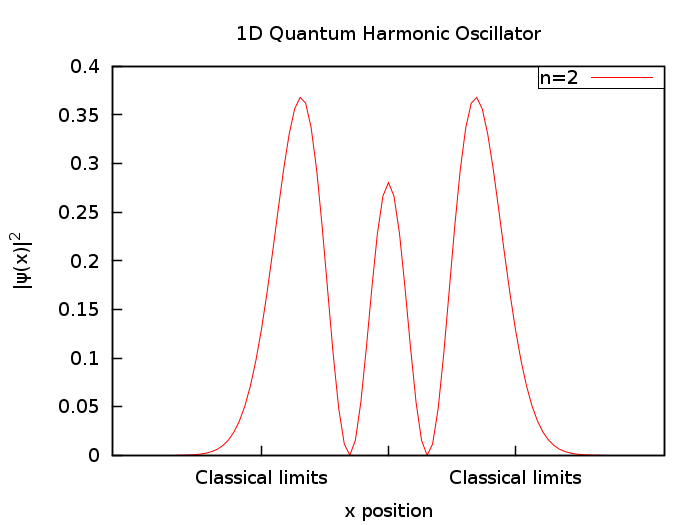
\includegraphics[width=3.35in]{harmOsc2n.png}
 % harmOsc.png: 0x0 pixel, 300dpi, 0.00x0.00 cm, bb=
 \caption{\it \small{The probability density of a particle in the $n$=2 state}}
 \label{fig:harmOsc2n}
\end{figure}
\newpage
An interesting feature of FIG.~\ref{fig:harmOsc2n} is that the particle has a nonzero probability to be outside the 
energetically allowed region for a classical harmonic oscillator, which allows for the particle to ``tunnel" through 
energetic barriers under the right conditions. This phenomenon has been well documented, and is the basis for technological 
innovations such as the Scanning Tunneling Microscope (STM)~\cite{STM}. 

\subsection{Two-dimensional, time-independent case.}

The Schr\"{o}dinger equation for a two-dimensional, time-independent, quantum harmonic oscillator is:
\begin{equation}
\psi^{(2)}(x,y) = -\frac{2m}{\hbar}[E-V(x,y)]\psi(x,y) \label{2DHO}
\end{equation}
where the potential is~\cite{mathjournal}:
$$V(x,y) = \frac{1}{2}m(\omega_{x}^2 x^2 + \omega_{y}^2 y^2)$$
and the total energy is~\cite{mathjournal}:
$$E = (n_{x} + \frac{1}{2})\hbar \omega_{x} + (n_{y} + \frac{1}{2})\hbar \omega_{y}.$$
Such a potential and total energy is analogous to that of two independent one-dimensional harmonic 
oscillators.  For this reason they were expected and verified to produce values twice as large as their 
one-dimensional counterparts.


\begin{figure}[H]
  \begin{center}
\centerline{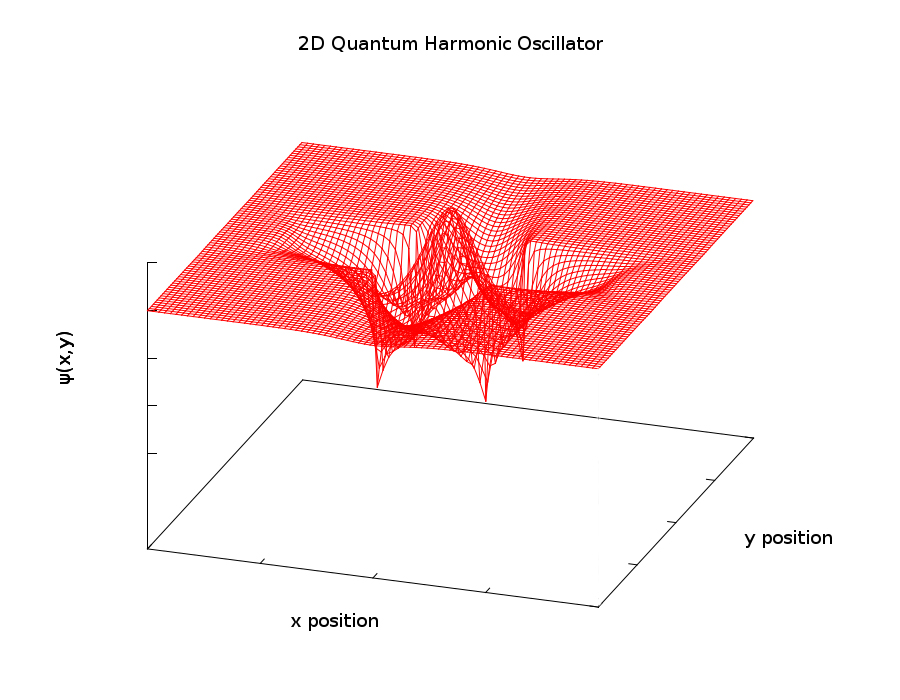
\includegraphics[width=3.35in]{2D_psi.png}}
\caption{\it \small{The wavefunction of a particle in a potential well, associated with the third bounded eigenstate, $n$=2, as generated by Numerov's algorithm \label{2Dpsi_n2}}}
  \end{center}
\end{figure}

FIG.~\ref{2Dpsi_n2} is a graph of $\psi(x,y)$ at its third bounded eigenstate.  As expected from FIG.~\ref{fig:harmOsc}, 
the wavefunction is symmetic about the x-axis.  It is also apparent that the wavefunction displays symmetry about the y-axis.  
This is to be expected based of the analog of the two-dimensional case being the same as two independent one-dimensional 
harmonic oscillators.


This allows us to explicitly define the two-dimensional wave function~\cite{mathjournal}:
\begin{center}
$\psi(x,y) = \sqrt{\frac{2^{-(n_{x}+n_{y})}}{n_{x}!n_{y}!}} * (\frac{m^{2}\omega_{x}\omega_{y}}{\pi^{2}\hbar^{2}})^{\frac{1}{2}} * exp({\frac{-m(\omega_{x}x^{2} + \omega_{y}y^{2})}{2\hbar}}) * H_{n_{x}}(\sqrt{\frac{m\omega_x}{\hbar}}x) * H_{n_{y}}(\sqrt{\frac{m\omega_y}{\hbar}}y)$
\end{center}
\newpage
\begin{figure}[htb!]
  \begin{center}
\centerline{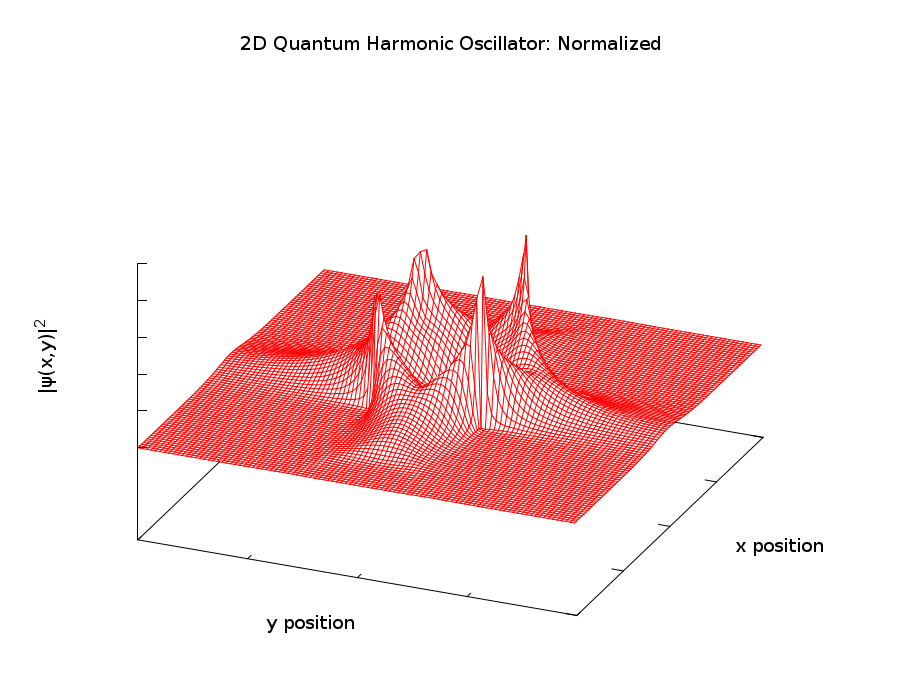
\includegraphics[width=3.35in]{2D_psisquared.png}}
\caption{\it \small{The probability density of a particle in a potential well, associated with the third bounded eigenstate, $n$=2, as generated by Numerov's algorithm \label{2Dpsi2_n2}}}
  \end{center}
\end{figure}

FIG.~\ref{2Dpsi2_n2} depicts $|\psi(x,y)|^2$ at its third bounded eigenstate.  Here $|\psi(x,y)|^2$ has 2 nodes in the x-direction
and 2 nodes in the y-direction, as does the corresponding wavefunction represented in FIG.~\ref{2Dpsi_n2}.




Shown in FIG.~\ref{2Dpot} is a two-dimensional potential well, used in Numerov's algorithm to generate wavefunctions.  This well is for a two-dimensional 
harmonic oscillator.  Within the well is the classically allowed region in which a paticle can reside.  Outside this well 
represents the ``forbidden regions" - regions a particle is not allowed to exist under classical conditions.  It is expected 
that a particle's position probability density will be zero at all places it is forbidden.  Yet it has been shown that this 
is not always the case.  This phenomenon is known as tunneling, as discussed above.
 

\begin{figure}[H]
  \begin{center}
\centerline{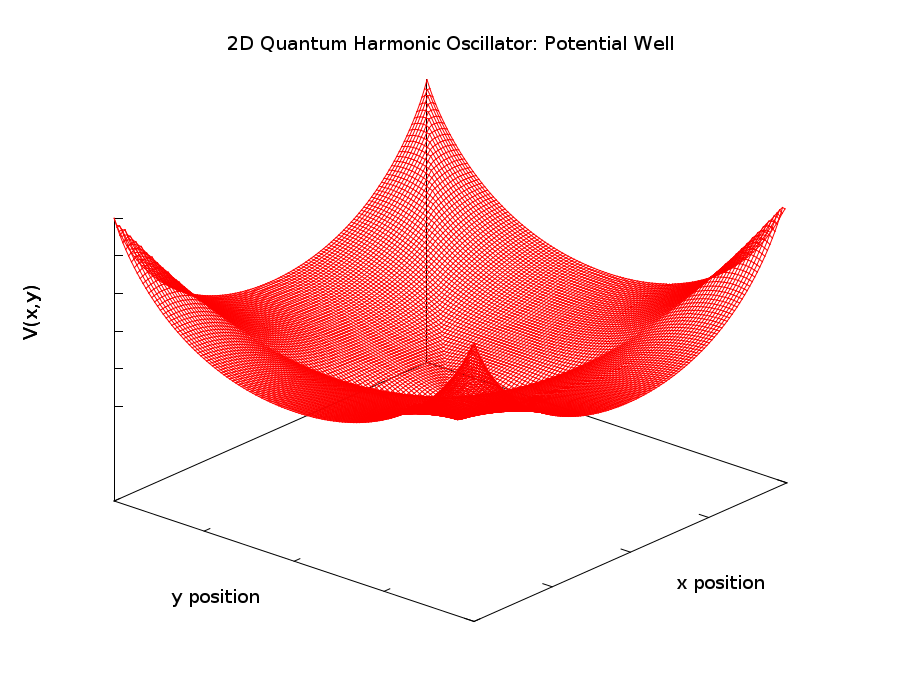
\includegraphics[width=2.7in]{2D_potentialwell_wo.png}}
\caption{\it \small{A two-dimensional potential well, used in Numerov's algorithm to generate wavefunctions \label{2Dpot}}}
  \end{center}
\end{figure}

The potential well is the same for all bounded eigenstates of a quantum harmonic oscillator.  Although FIG.~\ref{2Dpot} does 
not change, the wavefunction and probability density do.  FIG.~\ref{four} shows the wavefunction a particle trapped in 
such a potential well, for its fifth bounded eigenstate.

\begin{figure}[h!]
  \begin{center}
\centerline{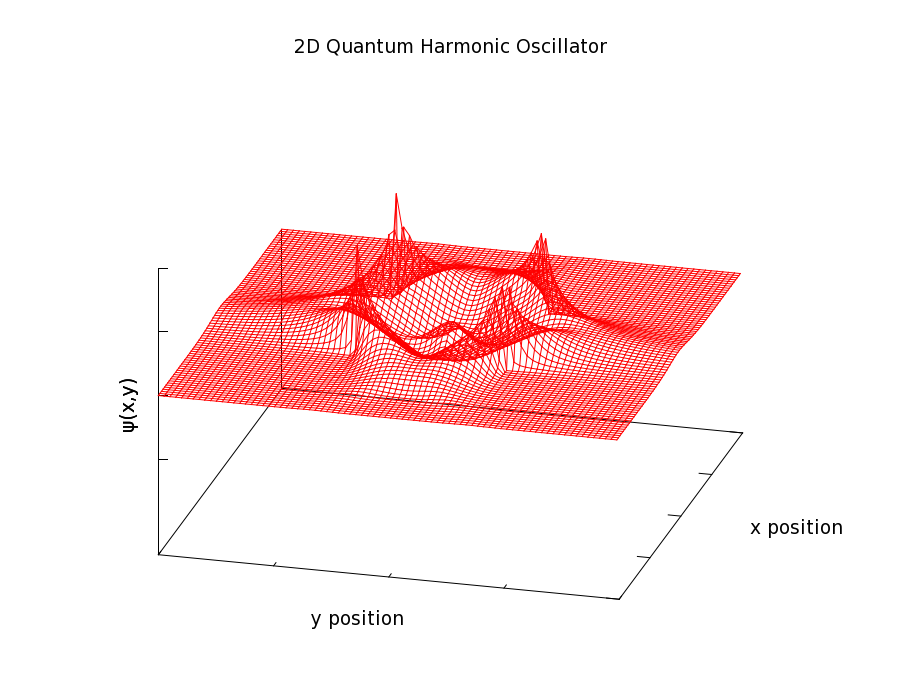
\includegraphics[width=3.35in]{2D_psi_n4.png}}
\caption{\it \small{The wavefunction of a particle in a potential well, associated with the fifth bounded eigenstate, $n$=4, as generated by Numerov's algorithm \label{four}}}
  \end{center}
\end{figure}

In a similar fashion FIG.~\ref{four2} shows a particle's position probabilty density, associated with the fifth bounded eigenstate.

\begin{figure}[h!]
  \begin{center}
\centerline{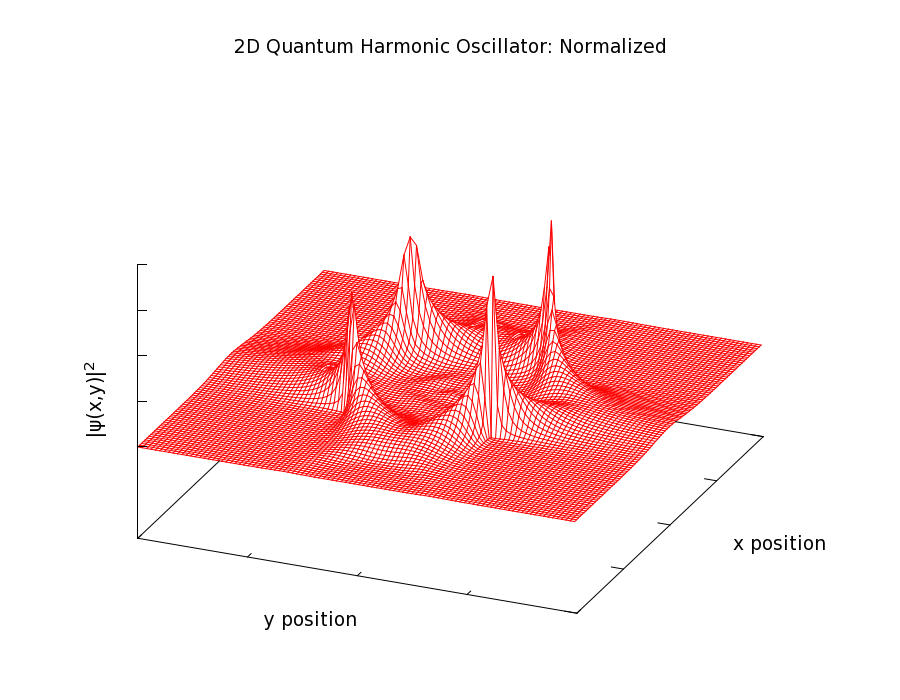
\includegraphics[width=3.35in]{2D_psisquared_n4.png}}
\caption{\it \small{The probability density of a particle in a potential well, associated with the fifth bounded eigenstate, $n$=4, as generated by Numerov's algorithm \label{four2}}}
  \end{center}
\end{figure}

\section{Results and Analysis}

Ultimately, we want to apply these techniques to make an accurate model of real physical systems. An infinite square well potential, as well as the parabolic potential described in the harmonic oscillator case can make approximations of the potential energy function experienced by an electron around a proton. In reality, the hydrogen experiences a radially symmetric coulombic potential:
\begin{equation}
 V(r) = -\frac{e^2}{4\pi\epsilon_0r}	\label{coulomb}
\end{equation}
Where $e$ is the elementary charge, and $\epsilon_0$ is the vacuum permittivity.  Setting constant $e^2/4\pi\epsilon_0 \equiv q_e$ the potential is:
\begin{equation}
 \frac{q_e^2}{r}	\label{coulomb2}
\end{equation}
The energy levels of this system are~\cite{code}:
\begin{equation}
 E_n = -\frac{m_eq_e^4}{2\hbar^2}\frac{1}{n^2}
\end{equation}The negative energy level in this case describes the binding energy of the electron to the proton. The energy goes like -1/n, so in general electrons with a lower quantum state have a greater binding energy. The wavefunctions generated by Numerov's algorithm of several bound states in a hydrogen atom are shown below: 
\begin{figure}[h!]
  \begin{center}
\centerline{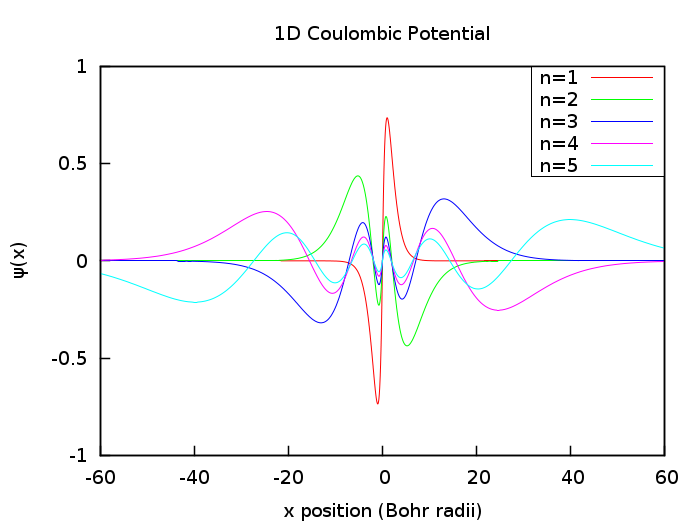
\includegraphics[width=3.35in]{hydrogen.png}}
\caption{\it \small{The wavefunctions of the first five bound energy states in a hydrogen atom. \label{hydrogen}}}
  \end{center}
\end{figure}
\begin{figure}[h!]
  \begin{center}
\centerline{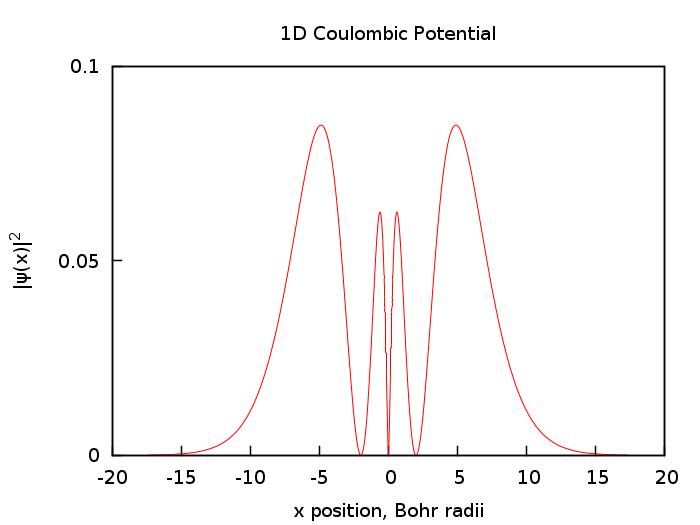
\includegraphics[width=3.35in]{radial2n.png}}
\caption{\it \small{The probability density associated with the $n=2$ energy state in a hydrogen atom. \label{hydrogen}}}
  \end{center}
\end{figure}
\begin{table}[h!]
\label{data}
\begin{center}
\begin{tabular}{|c|c|c|c|} 
\hline
n  & Predicted $E_n$, eV  & Simulated $E_n$, eV   & Fractional Error \\
\hline\hline
1  & $-13.6058000$ & $-13.6058000$ & $0.0$\\
\hline
2  & $-3.40145000$ & $-3.40145000$ & $0.0$\\
\hline
3  & $-1.51175556$ & $-1.51175556$ & $0.0$\\
\hline
4  & $-0.850362504$ & $0.850362500$ & $1.05\times10^{-8}$\\
\hline
5  & $-0.544231330$ & $0.544232000$ & $1.2\times10^{-7}$\\
\hline
\end{tabular}
\caption{\it\small{Comparison of simulated and predicted eigenvalues in the hydrogen atom}}
\end{center}
\end{table}
\newpage
The benefit of the numerical approach is that we can also apply these methods to cases which are difficult or in some cases can not currently be solved by analytical methods. For example, we can model the wavefunction of an electron near a diatomic molecule such as H$_2$. There are several approximations being made here; we take only the principle quantum number $n$ into account, thus angular momentum, quantum spin and magnetization are neglected. Additionally, we neglect the bonded pair of electrons shared by the 
H$_2$ molecule, which would contribute to the potential energy function in that region. As currently written, our code is also only able to produce stable waveforms for certain conditions. A wavefunction for an energy state with four nodes, and the corresponding probability density is shown below: 
\newpage
\begin{figure}[h!]
  \begin{center}
\centerline{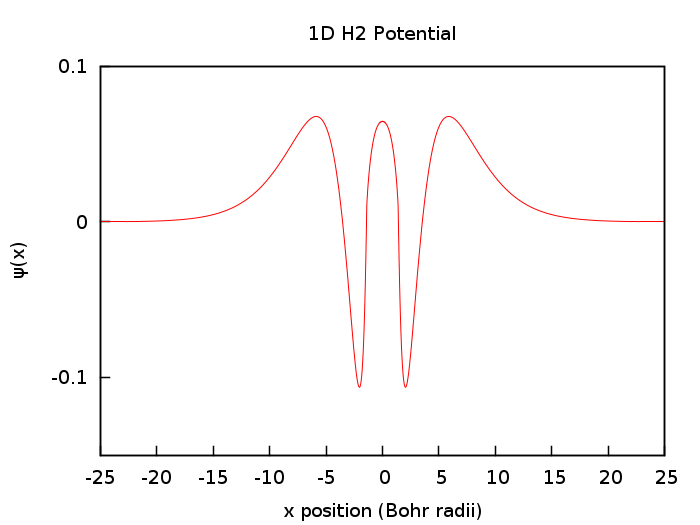
\includegraphics[width=3.35in]{H2.png}}
\caption{\it \small{The wavefunction of an electron near a diatomic hydrogen molecule. \label{hydrogen}}}
  \end{center}
\end{figure}
FIG~\ref{hydrogen} shows the wavefunction of an electron in the vicinity of a diatomic hydrogen molecule. The wavefunction does converge to reasonable results away from the origin, but it's difficult to interpret if it describes a state which could physically occur. For instance, FIG~\ref{hydrogenprob} below shows the probability density of this wavefunction, but we see peaks near the origin. Neglecting the influence of the bonded electron pair in the molecule could explain this non-physical result generated by our program. 
\begin{figure}[h!]
  \begin{center}
\centerline{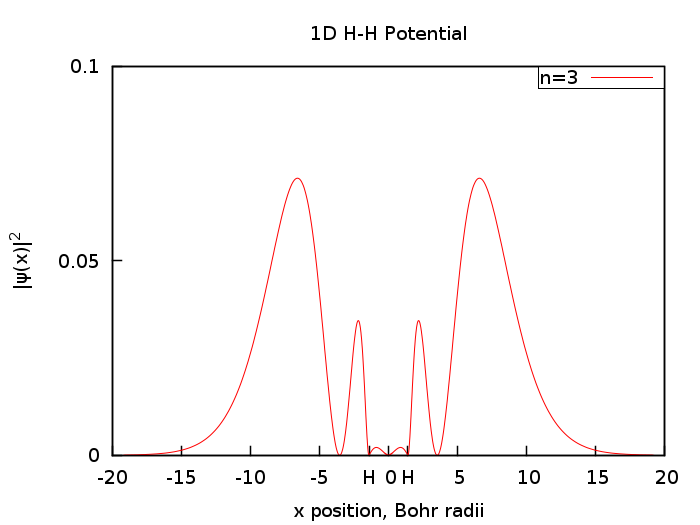
\includegraphics[width=3.35in]{H22n.png}}
\caption{\it \small{The probability density of an electron near a diatomic hydrogen molecule. \label{hydrogenprob}}}
  \end{center}
\end{figure}
\newpage
\section{Conclusions}

Computational analysis of the Schr\"{o}dinger wave equation is no easy task.  Once achieved, numerical methods are able to 
assist us in obtaining otherwise unachievable results.  It is necessary to first model a system with a known outcome, to 
insure the written program functions properly.  Only then is it possible to extrapolate the methodolgy and apply it to 
systems that are not analytically solvable.  This results in an understanding of the system otherwise unachievable.

Computational modeling allows the visualization of such physical phenomenon.  Simulations aide our understanding by not only allowing us to 
see the scenario we are describing but also make predictions.  Predictions whos accuracy would otherwise not be established.



\setlength{\parindent}{0cm}

\begin{thebibliography}{99}  % the trailing 99 controls some obscure format--just use

\bibitem{Sch_eq} Weisstein, Eric W. ``Schr\"{o}dinger Equation."
{\em Schr\"{o}dinger Equation. } Mathematica, 1996. Web. 2 May 2015.

\bibitem{Javapsi} Schmittfull, Marcel. ``Simulating and Visualizing Quantum Mechanics."
{\em JavaPsi. } (n.d.):n. pag. Celtis-Gymnasium Schweinfurt. Web. 2 May 2015.

\bibitem{Schrodinger_wave} ``Erwin Schrödinger - Biographical". {\em Nobelprize.org. } Nobel Media AB 2014. Web. 8 May 2015.

\bibitem{comparison} Norton, Matthew S. ``Numerov's Method for Approximating Solutions to Poisson's Equation." (2009): n. pag. 2009. Web. 3 May 2015.

\bibitem{STM} Chen, Julian C. ``Introduction to Scanning Tunneling Microscopy" Web. 3 May 2015.

\bibitem{mathjournal} Mahasneh, Abdallah, Safwan Al-Shara', and A. M. Al-Qararah. 
    ``Solution of Time-Independent Schrodinger Equation for a Two-Dimensional Quantum Harmonic Oscillator 
    Using He's Homotopy Perturbation Method." {\em Journal of Mathematics Research} 3.2 (2011): n. pag. Web. 5 May 2015. 

\bibitem{code} Lennard-Jones, J. E. ``Perturbation Problems in Quantum Mechanics." {\em Proceedings of the Royal Society of London. 
      Series A} Containing Papers of a Mathematical and Physical Character.Vol. 129, No. 811 (1930): 598-615. Web. 3 May 2015. 

\end{thebibliography}


\end{document}

